\section{Gaussian Mixture Model}
\label{sec:gaussian}
A Gaussian Mixture Model is a probabilistic model that assumes that the data are generated from a mixture of several gaussian distributions. Depending on the parameters of a Gaussian distributions (mean and variance) it the data generated from it will have a shape that resamble an elipsoid with a centre and a orientation.
 

\begin{figure}[htbp]
    \centering
    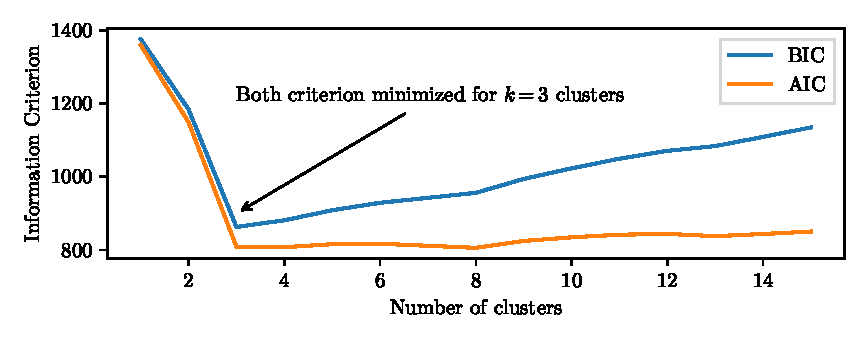
\includegraphics{images/Gaussian/Figure_1.pdf}
    \caption{Criteria for selecting the number of clusters}
    \label{fig:gauss_criterion}
\end{figure}

\begin{figure}[htbp]
    \centering
    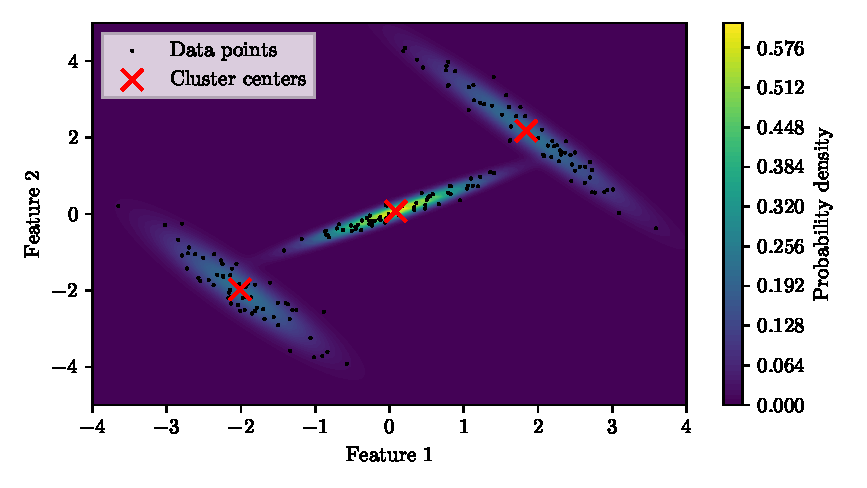
\includegraphics{images/Gaussian/Figure_2.pdf}
    \caption{Trained Gaussian Mixture Model}
    \label{fig:gauss_example}
\end{figure}